\section{evaluation}
\label{sec:eval}
We measured various performance aspects of Camelot to measure its
scalability and competitiveness with existing data processing
platforms. We developed a set of benchmark programs with diverse
memory access patterns, to measure the quality of our page eviction
strategies, threading performance, and raid overhead.
\begin{figure*}[h]
	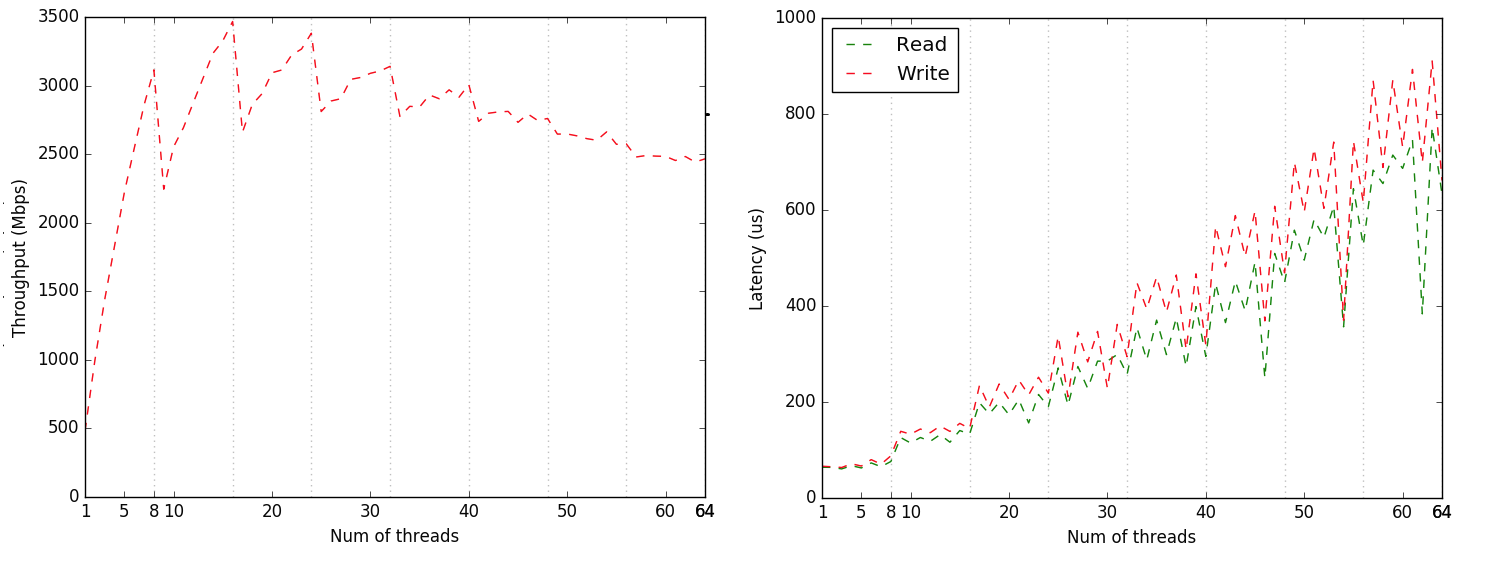
\includegraphics[width=\textwidth]{fig/threads_pinned}
	\caption{Microbenchmarks of the Camelot request API. The two figures show latency and throughput 
	with threads pinned to cores in round-robin fashion.}
	\label{fig:threads}
\end{figure*}
\subsection{Experimental setup}
Our tests were performed in the Mininet~\cite{mininet} as well as on real hardware.
Mininet is a host-local network emulator intended to rapidly prototype SDN and data center network environments. Mininet allow us to verify and deploy code quickly, without having to worry about hardware constraints or configuration. While absolute performance may not exactly be accurate, relative improvements are generally reliable. 
Our real hardware setup consisted of three servers, each of which is equipped with a 10-Gigabit X540-AT2 NIC, 32 GB of memory, and two four-core Intel(R) Xeon(R) E5-2407 v2 CPUs. The cores do not support hyperthreading.
The microbenchmarks and threading tests were performed on real hardware to provide an accurate picture of the current system efficiency. The remaining tests were run in Mininet, as absolute performance was not of concern.

\subsection{Threading Performance}
To understand the implications of multithreading, and to verify the functionality of our current networking stack, we conducted several microbenchmarks. We pinned each thread to one core in a round-robin fashion, as this approach has proven itself to be more stable and reliable during testing. Our benchmark consisted of a million read and write requests, which we then scaled up to 64 threads. The results are shown in Fig~\ref{fig:threads}.
As expected, throughput scales linearly up to eight threads and latency does not increase. Unfortunately, the program is unable to exhaust the NIC bandwidth and only reaches around 3.5 out of 10 Gbit per second. At the same time, while latency in Mininet is on the order of ~9-10 microseconds, real RTT is ~60-70. This caused by a lack of request batching and the use of slow kernel networking code.

We decided to go beyond the expected scaling of eight cores and explore the system behaviour up to 64 threads. The pinned experiment ran stable, demonstrating a reasonable reliability. The throughput results exhibit a sawtooth pattern, with a local maximum occurring  every eighth thread. This pattern is caused by the number of cores and pinning. However, this does not explain the maxima achieved by 16 and 24 threads. We assume that these may be caused by batching of requests in the NIC buffer, which is beneficial for throughput.
Latency behaves as expected, with a mild increase in early iterations that transitions into wild instability the more threads are added.

\subsection{Paging Performance}
The purpose of our page performance evaluation was to quantify the performance improvement over the BlueBridge paging policy and to determine which paging policy is most efficient. Our first benchmark was running PageRank with varying amounts of local memory and each paging policy. The entire runtime is measured on the Google web graph dataset, roughly 75MB. The second benchmark was sorting a large number of random integers with varying local memory amounts.

\begin{figure}[H]
    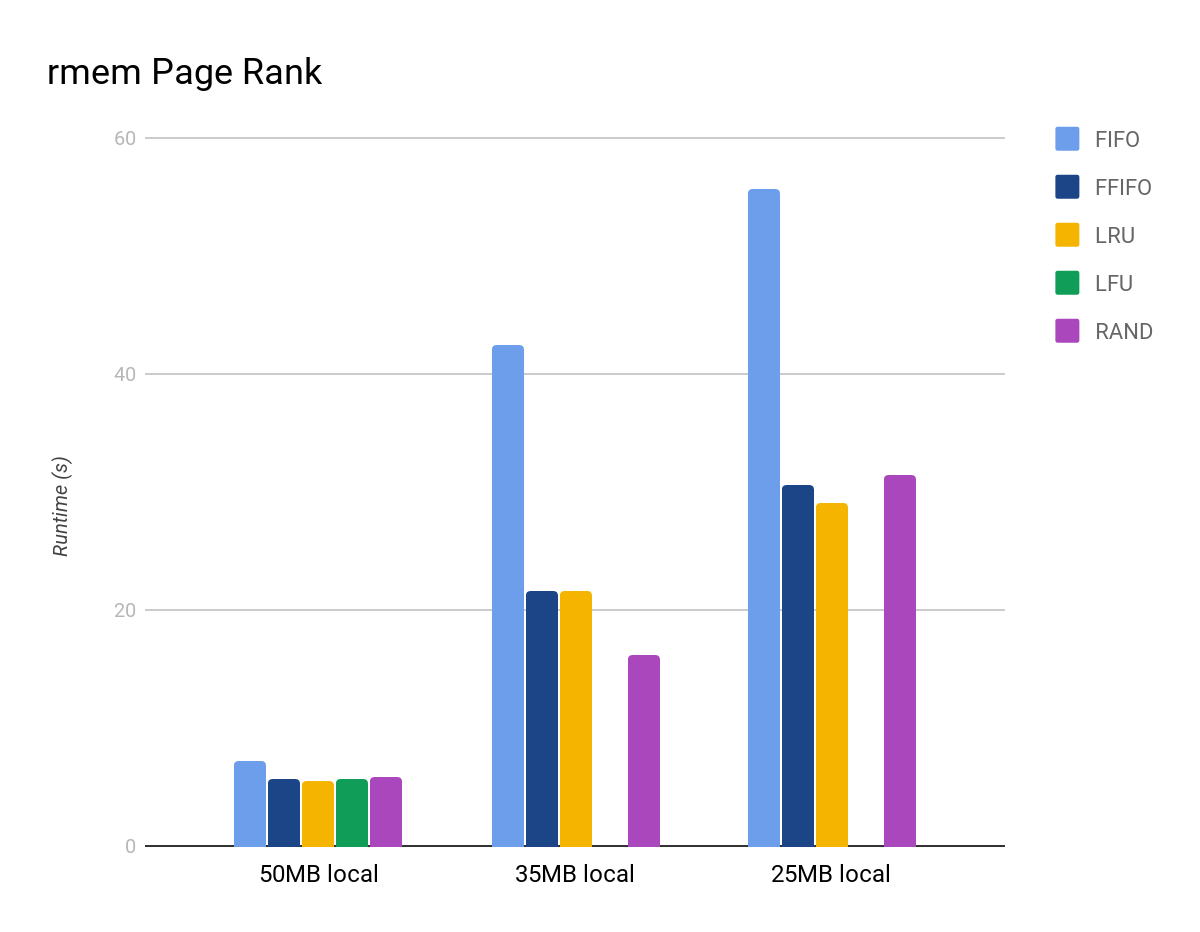
\includegraphics[width=\columnwidth]{fig/policyPerformance}
    \caption{PageRank runtime benchmark for each policy with decreasing amount of local memory.}
    \label{fig:policyPerformance}
\end{figure}

In the Pagerank benchmark, the LRU and improved FIFO policies outperformed the existing FIFO regardless of local memory size, achieving nearly half the execution time in the 35MB and 25MB tests as shown in Fig~\ref{fig:policyPerformance}. As local memory was limited and more page replacements were made, the LFU eviction policy failed to replace the correct pages and execution time increased dramatically, the results of which for 35MB and 25MB local memory were 9 minutes and 40 minutes respectively. To test the effectiveness of the policies, a random replacement policy was implemented. Ideally there would have been a substantial performance benefit from using the new replacement policies over the random replacement but the random replacement policy performed the best in the 35MB local memory test and still performed reasonably well with 50MB and 25MB. This is could be due to the policies implemented being based only on write usage as the nodes are moved around on segfault. For further work it would be beneficial to capture the read usage in an efficient way for the LRU and LFU policies.

\begin{figure}[H]
    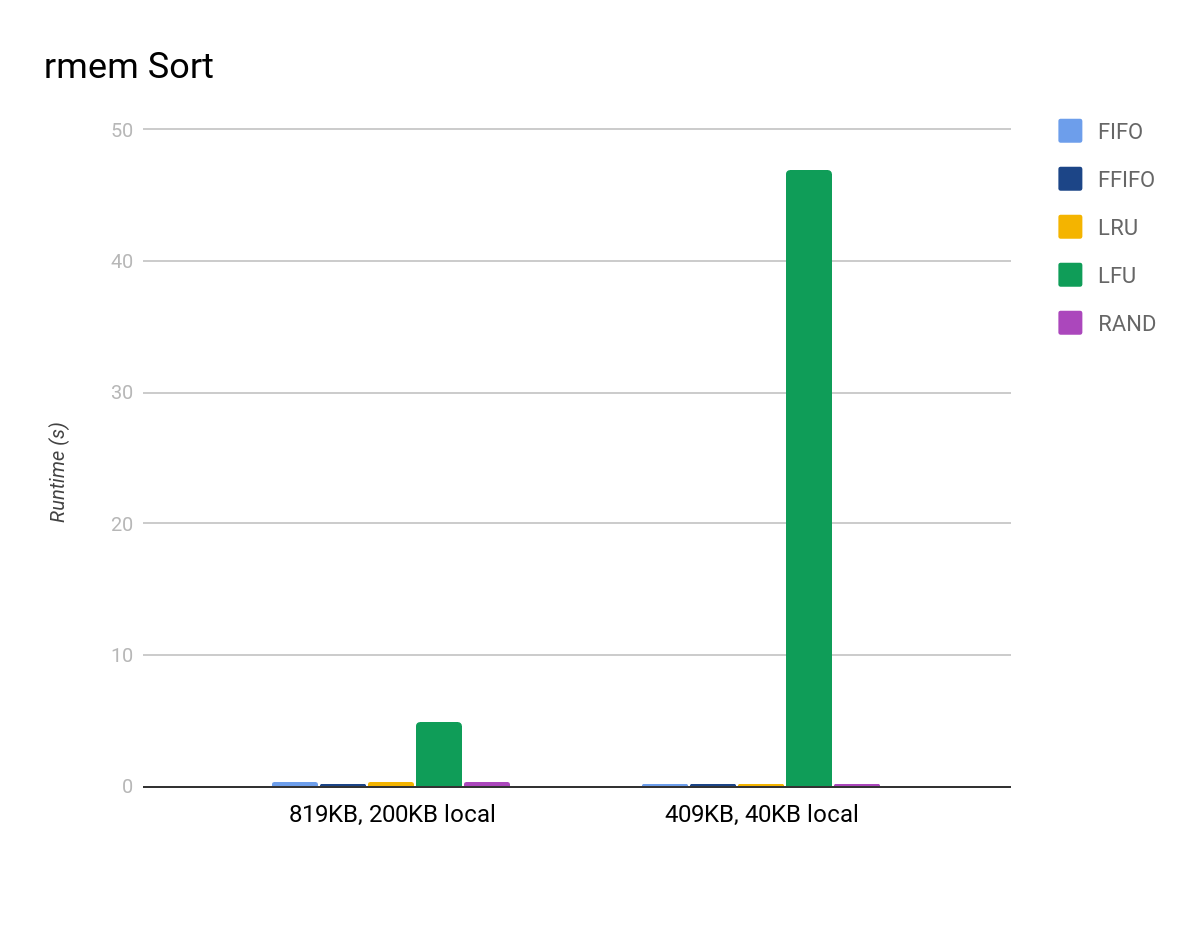
\includegraphics[width=\columnwidth]{fig/sortPerformance}
    \caption{Sort runtime benchmark with decreasing amount of local memory for each policy.}
    \label{fig:sortPerformance}
\end{figure}

In the Sort benchmark the existing FIFO and new replacement policies performed similarly with the exception of LFU. The results of the Sort benchmark in Fig~\ref{fig:sortPerformance} show the extreme difference between having a large number of local pages and a small number of local pages when using LFU.

\subsection{RAID Overhead}

Our goal in evaluating our RAID implementations is twofold. We first
wished to establish a baseline overhead of running raid over regular
remote memory, and to compare the cost of parity calculation relative
to the no parity case common to RAMCloud. In both cases we found that
the size of local cache used dramatically affected performance, so we
report our performance results as a function of local cache size. We
measured relative performance of these algorithms by timing
iterations of a single threaded PageRank algorithm. Each iteration
of page rank requires both a read and write step, so in each
iteration all pages are read, and written to remote memory.

\begin{figure}[H]
    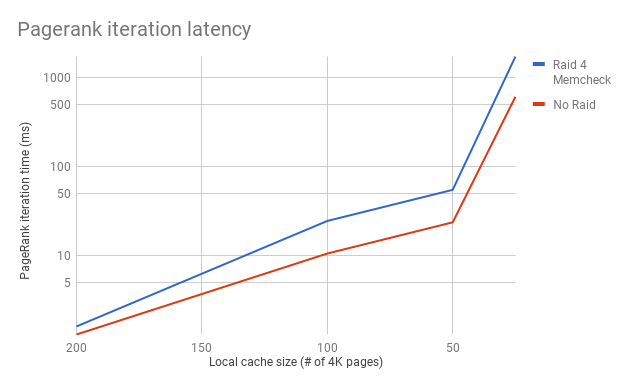
\includegraphics[width=\columnwidth]{fig/Raid4Overhead}
    \caption{A logarithmic plot of RAID 4 running with memory check performed on reads, and parity calculations on writes, v.s traditional remote memory.}
    \label{fig:raid4Overhead}
\end{figure}

We found that running RAID4 with memory correction on a small local
cache 1-2\% of the entire graph) caused a 2x slowdown in PageRank
iterations. The relation between performance and local cache size is
plotted in Figure~\ref{fig:raid4Overhead}. As the number of local
pages was increased to 10-20\% of the entire graph the overhead was
reduced to ~1.5x slowdown. A large component of this overhead, is not
the cost of performing XOR, it is due to our networking stacks lack of
optimization for RAID. Our RAID manager is build directly on top of
our remote memory stack, which issues single requests in the form of 4K
pages. Therefore RAID 0,4,5 increase network bandwidth by $(n-1)x4K$
per page. Batching requests, and optimizing the network stack to
read/write stripes of pages will substantially drop overhead.

\begin{figure}[H]
    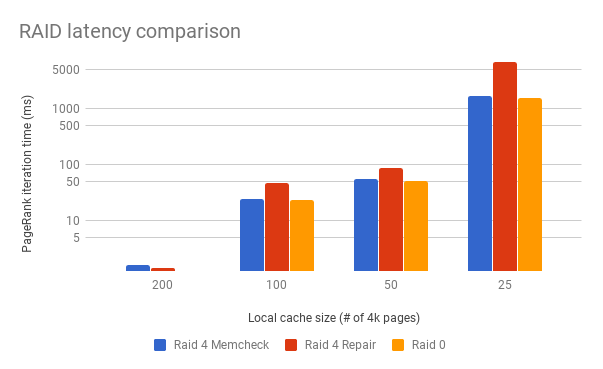
\includegraphics[width=\columnwidth]{fig/RaidComparison}
    \caption{Raid 4, Raid 4 with failure, and Raid 0 vs local cache size}
    \label{fig:RaidComparison}
\end{figure}

To evaluate the relative performance of RAID 4 \& 5 compared to RAID
0 \& 1 we likewise measured PageRank iteration times. We found that
Raid 4 and 5 introduce a 6\% overhead on both RAID 0 \& 1, and that
the overhead was directly proportional to parity calculation time.
Figure~\ref{fig:RaidComparison} plots our comparative results. RAID 0
\& 1 ran competitively within 0.01\% of each other. The only notable
difference between then was the lack of a need for RAID 1 to wait for
stragglers on reads. Given our setup the straggler problem was
unobservable to our measurements. RAID 4 \& 5 operate identically from
a latency and bandwidth perspective. We also measured the performance
penalty from running during a failure. We killed a single memory
server while running PageRank and observer the overhead to be
approximately 2x. The majority of the overhead was caused by waiting for
a preset 100 microsecond timeout to fire and initiate the repair
calculation. This overhead could be reduced by introducing a failure
detector which would initiate repair immediately. In this case the
overhead of running Camelot on 3 memory nodes under failure, vs
RAMCloud is 6\% while requiring 50\% of the total memory.

